\documentclass{article}
%%\documentclass[journal=jctcce,manuscript=article,layout=twocolumn]{achemso}
%%\usepackage[version=3]{mhchem} % Formula subscripts using \ce{}
%\usepackage{achemso}
%\setkeys{acs}{articletitle = true}
\usepackage{graphicx} % for EPS, load graphicx instead
\usepackage{url}      % llt: nicely formatted URLs
\usepackage[sorting=ydnt]{biblatex}
\addbibresource{molecularDynamics.bib}
\usepackage[hmargin=3cm,vmargin=3.5cm]{geometry}

%%%%%%%%%%%%%%%%%%%%%%%%%%%%%%%%%%%%%%%%%%%%%%%%%%%%%%%%%%%%%%%%%%%%%
%% If issues arise when submitting your manuscript, you may want to
%% un-comment the next line.  This provides information on the
%% version of every file you have used.
%%%%%%%%%%%%%%%%%%%%%%%%%%%%%%%%%%%%%%%%%%%%%%%%%%%%%%%%%%%%%%%%%%%%%
%%\listfiles

%%%%%%%%%%%%%%%%%%%%%%%%%%%%%%%%%%%%%%%%%%%%%%%%%%%%%%%%%%%%%%%%%%%%%
%% Place any additional macros here.  Please use \newcommand* where
%% possible, and avoid layout changing macros (which are not used
%% when typesetting).
%%%%%%%%%%%%%%%%%%%%%%%%%%%%%%%%%%%%%%%%%%%%%%%%%%%%%%%%%%%%%%%%%%%%%
\newcommand*{\mycommand}[1]{\texttt{\emph{#1}}}

%%%%%%%%%%%%%%%%%%%%%%%%%%%%%%%%%%%%%%%%%%%%%%%%%%%%%%%%%%%%%%%%%%%%%
%% Meta-data block

%% ---------------
%% Each author should be given as a separate \author command.
%%
%% Corresponding authors should have an e-mail given after the author
%% name as an \email command.
%%
%% The affiliation of authors is given after the authors; each
%% \affiliation command applies to all preceding authors not already
%% assigned an affiliation.
%%
%% The affiliation takes an option argument for the short name.  This
%% will typically be something like "University of Somewhere".
%%
%% The \altaffiliation macro should be used for new address, etc.
%%%%%%%%%%%%%%%%%%%%%%%%%%%%%%%%%%%%%%%%%%%%%%%%%%%%%%%%%%%%%%%%%%%%%
\author{Jos\'e O. Sotero-Esteva \\
Department of Mathematics\\
University of Puerto Rico at Humacao\\
Humacao, Puerto Rico\\
jose.sotero@upr.edu}
\title
{Wolffia: An environment with a graphical user interface to prepare and monitor classical molecular dynamics simulations}
\begin{document}

\maketitle
%%%%%%%%%%%%%%%%%%%%%%%%%%%%%%%%%%%%%%%%%%%%%%%%%%%%%%%%%%%%%%%%%%%%%
%% The document title should be given as usual
%% A short title can be given as a *suggestion* for running headers.
%%%%%%%%%%%%%%%%%%%%%%%%%%%%%%%%%%%%%%%%%%%%%%%%%%%%%%%%%%%%%%%%%%%%%


\begin{abstract}
\textit{Wolffia} is a software environment to prepare and monitor classical molecular dynamics simulations (CMD) with a design based on well established graphical user interface principles. This has lead to an
arrangement of tools in sections intended to support the user 
throughout the simulation process: building a system, configuring force fields, defining periodic boundary conditions and solvating, 
energy minimization, and the simulation of the dynamics. It provides utilities not just for creating, editing and 
displaying molecular systems but also to allow the user to run simulations by using a widely used simulation program, as it automatically assembles the configuration 
settings for doing so.
Test cases demonstrate that, as a result, this software is capable of easily producing CMD simulations results on current research subjects proving that it effectively addresses the needs of people with knowledge ranging from pre-university level through researchers.
Wolffia is open-source and its latest release is available at \texttt{http://wolffia.uprh.edu}. 
 
\end{abstract}
%%%%%%%%%%%%%%%%%%%%%%%%%%%%%%%%%%%%%%%%%%%%%%%%%%%%%%%%%%%%%%%%%%%%%
%% Start the main part of the manuscript here.
%%%%%%%%%%%%%%%%%%%%%%%%%%%%%%%%%%%%%%%%%%%%%%%%%%%%%%%%%%%%%%%%%%%%%



\section{Introduction}

The main purpose of \textit{Wolffia} is to serve as an integrated tool to perform molecular dynamics simulations by
providing a clean and simple but effective graphical user interface to the process of setting-up such simulations.  
It has been built based on established human-computer interface (HCI) principles.  With it, inexperienced  as well as experienced users 
can build molecule systems using several molecular data input methods combined with a simple atom by atom editing tool.  With its force field tool, the user may comfortably set parameters and/or infer them based on publicly available data.
It relies on a well established general-purpose 
CMD simulator for the potential minimization and dynamics simulations as well as on several other libraries known and used by many researchers and educators who use classical molecular dynamics.  
Its supporting website provides the necessary tools to facilitate collaboration of the CMD community interested in enhancing its capabilities.

The descriptions made here correspond to version 1.

\begin{table}
  \label{tbl:abbreviations}
  \begin{tabular}{ll}
    \hline
    \textbf{Abbreviation}  & \textbf{Meaning}\\    
    \hline
	CHARMM & \textit{Chemistry at HARvard Molecular Mechanics} (application and force field format)\\
	CMD  & Classical molecular dynamics \\
	CNT    & Carbon nanotube\\
	GUI    & Graphical user interface \\
	LAMMPS & \textit{Large-scale Atomic/Molecular Massively Parallel Simulator} (application)\\
	MAPS & \textit{Materials and Processes Simulations} (application) \\
	NAMD & \textit{Not (just) Another Molecular Dynamics} program (application)\\
	NCI-CADD & \textit{National Cancer Institute / Computer-Aided Drug Design Group} \\
	PDB    & \textit{Protein Data Bank}, also refers to the file format \\
	SDS    & Sodium dodecyl sulfate\\
	VMD  & \textit{Visual Molecular Dynamics} (application) \\
    \hline
  \end{tabular}
  \caption{Abbreviations frequently used in this paper.}
\end{table}


\section{Usability.} 
\textit{Wolffia} has been designed from its conception as an application to support the process of building a CMD simulation.  It has  rich set of visual tools and clues that are not present in other software for CMD.  It does not require knowledge of technical details of internal formatting or coding schemes while allowing experienced users to use that knowledge if needed.  For example, fixing molecules is achieved by clicking on a pin widget, not editing PDB files or providing segment identifications.  Undo and redo buttons allow users to recover from most actions.  
Dealing with configuration and data files has been kept as hidden as possible from the user allowing him or her to focus on the chemical physics.  The time to set-up and run a small to medium sized simulation is reduced to minutes from hours or days when compared to manual manipulation of files or assisted with other GUIs for CMD tools that do not support the whole process.


\section{Details of the interface.}

In this section the main features of the program are described.  A test case of the simulation of a carbon nanotube (CNT) with Sodium dodecyl sulfate (SDS) surfactant similar to the one published recently by Duan \textit{et.al.} \cite{Collins2011} is used as an illustration.

The main section of the main GUI window (Figure \ref{fig:mainWindow}) has a collection of tabs ordered in a way that suggests the steps involved in the set-up of a MD simulation.  This may be used by a novice user as a guide without forcing a more experienced user into a linear design process.   The tabs are organized as follows: Build, Force Field, Container, Minimization, and Simulation.  A secondary section is used to track the changes in the system.  It consists of a molecule viewer and plots to track the energy and kinetics of the simulation.

In \textit{Wolffia}, a set of molecules is called a \textit{mixture}.  Its main window provides global tools that apply to all stages such as creating, deleting and/or switching between mixtures, resetting the current mixture, managing general settings, and saving/loading mixtures.  Undo and Redo buttons are also provided.



\subsection{Building the mixture.}
\textit{Wolffia} provides three essential tools in the \textit{Build} tab for generating and manipulating molecular structures: the \textit{Molecule Catalog}, the \textit{Structure Manager}, and the \textit{Property Editor}. The Molecule Catalog contains some commonly used structures such as allotrope (CNT, graphene), polymers, surfactants and others.  Complex structures such as CNT are constructed using a specialized editor in which the user specifies chirality, length, and others. Each editor has its own visualizer and a series of parameters needed for defining the attributes of the structure to be generated (figure \ref{fig:testCase} (a) and (c)). The \textit{Import Custom Molecule} option may be used as many times as needed to import existing structure files to \textit{Wolffia} in the form of coordinate and structure psf-files or by retrieving coordinate files directly from the \textit{Protein Data Bank} and NCI-CADD on-line sites.  

Figure \ref{fig:mainWindow} shows a CNT built using the \textit{CNT editor} surrounded by thirty five SDS molecules.  One SDS set of 
coordinates was imported from the NCI-CADD site into a separate mixture. Once the proper parameters were set and an initial minimization was performed on this molecule, copies of the SDS molecule were placed into the mixture with the CNT and set into their positions using the Property Editor in a few minutes.

One or many molecules can be selected by clicking on its name on the Molecule Manager and by clicking on the viewer as well.  The molecule manager serves to show or hide molecules from view and to fix molecules so that they stay frozen during a simulation.   
The build tab also has a limited capability for editing molecules that can be used, for example, to functionalize nanotubes  along with drilling and etching tools that can be used to build complex structures for nanotechnology applications as will be shown in the test case section below.

\begin{figure}
\begin{center}
  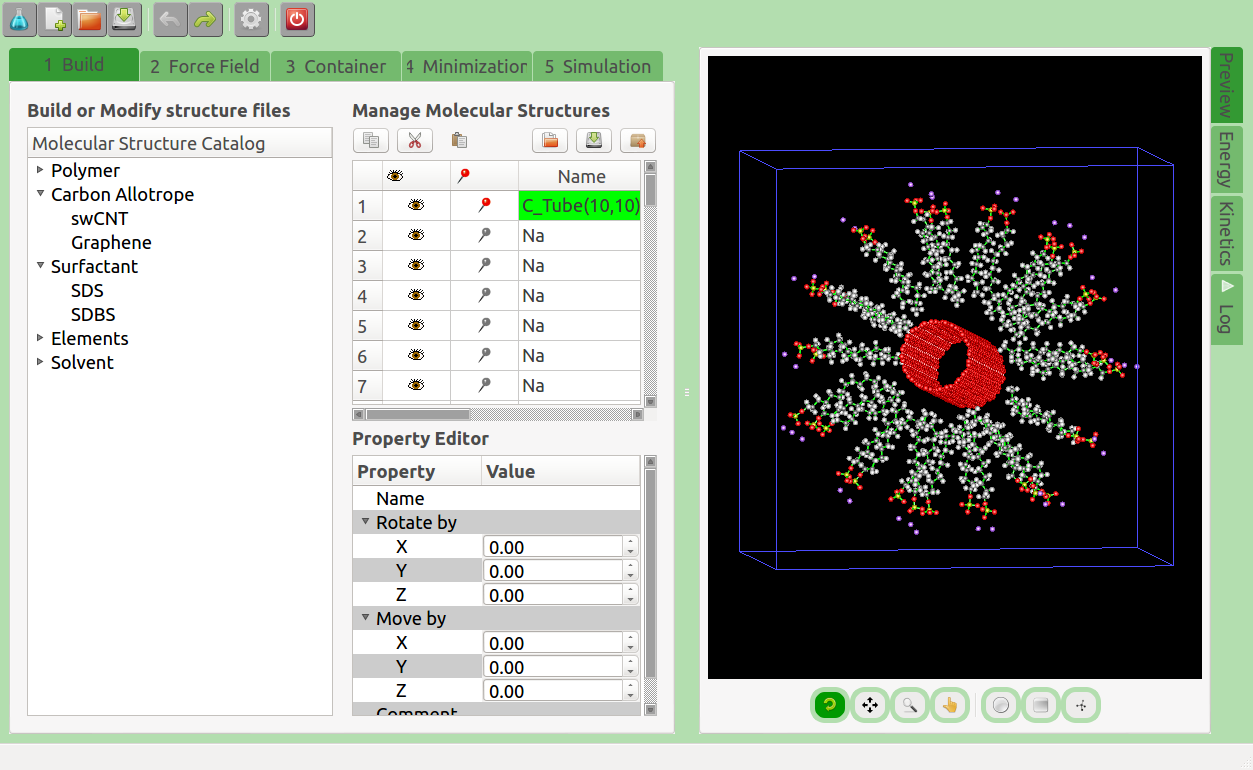
\includegraphics[scale=0.40]{mainWindow.png} 
  \caption{A single wall carbon nanotube built using the CNT editor surrounded by thirty five SDS molecules}
  \label{fig:mainWindow}

\end{center}\end{figure}



\subsection{Force Field editor.}
\textit{Wolffia} includes a mechanism for examining and modifying parameters for the Coulomb, non bonded, bonded, angle, and dihedral interactions (Figure \ref{fig:forceTab}). The parameters correspond to the force field given by the potential used by CHARMM
\[  \sum _ {bonds}  K_b(b-b_0)^2 + \sum _{angles} K_\theta (\theta-\theta_0)^2 +
 \sum_{dihedrals} K_\varphi (1+\cos(n\varphi-\delta))
\]
\[ + \sum_{iproper} K_\phi(\phi-\phi_0)^2 + \sum_{nonbonded} \left[ \frac{q_i q_j}{4\pi D r_{ij}} + \epsilon_{ij} \left [ \left (\frac{R_{min,ij}}{r_{ij}} \right)^{12} - 2 \left (\frac{R_{min,{ij}}}{r_{ij}} \right)^6 \right ]\right] \]
where $\epsilon_{ij} = \sqrt{\epsilon_{i}\epsilon_{j}}$, $R_{min,{ij}} = (R_{min,{i}} + R_{min,{j}})/2$.  The force tab provides separate sections to set the configurable parameters according their nature.  Nonbonded interactions require values for each atom type for the van der Waals radius $R_{min}$, its depth $\epsilon$ and the charge $q$ for Coulomb potential.  The bonds section is used to set the bond distance $b_0$ and stiffness $K_b$ for each pair of bonded atom types. The angles section has numeric fields for the angle $\theta_0$ and stiffness $K_\theta$ and the proper dihedrals section for the torsion angle $\delta$, its multiplicity $n$ and stiffness $K_\varphi$.  

Force field parameter values for the molecules built using the molecule catalog are automatically included.  References to the literature that validate those values appear in the files that can be browsed by the user.  Additional parameter values can be loaded from or stored into CHARMM-formatted force field files.  Since custom systems or molecules imported from on-line data banks have undefined force field values, those fields appear highlighted in yellow as a warning sign. 

A search mechanism for parameter values taken from publicly available CHARMM force fields is also provided.  It looks for structural matches between the user molecule and structures described in those files and responds with one that maximizes the number of parameters found.  The purpose of this mechanism is to set provisional values so that other parts of the MD simulation will work.  It can produce parameters values close to published ones, particularly for smaller molecules. For example, a search for values for a glycerol molecule downloaded from the NCI-CADD repository produces an exact match for Lennard Jones parameters extracted from  the C27r CHARMM force field as found in literature.\cite{Pastor}  But the user is warned that simulations performed with those parameters are not validated in any rigorous way and that the simulation results that use such parameters may fail to reflect actual physical behavior more often than validated ones.  In any case, force field parameters, even those obtained with sound molecular physics methods, should always be validated with experimental data or previously validated simulations.

Figure \ref{fig:forceTab} shows the angle parameters section for the force field of  the SDS molecule.  The mixture viewer has been set to show atom types. The potential for some angles is not defined and their corresponding values are zero and appear highlighted.  A simulation may run without some of those values.  Only the non-bonded potential parameters are required to be defined for all types of atoms.

\begin{figure}
\begin{center}
  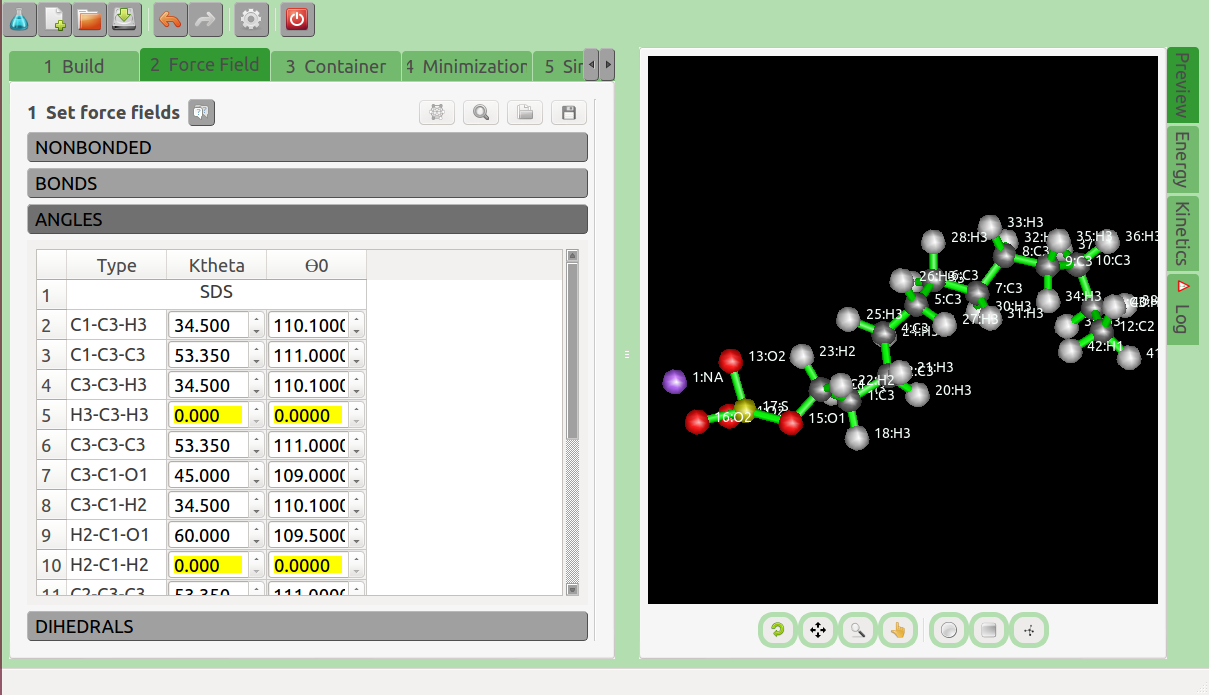
\includegraphics[scale=0.45]{forceTab.png} 
  \caption{The \textit{Force Field tab}.  Visual clues are used to draw attention to information that the researcher may need to define.}
  \label{fig:forceTab}
\end{center}
\end{figure}


\subsection{Container tab.}

Periodic boundary conditions and solvents to be used, if any, can be set using the tab shown in Figure \ref{fig:setupTab}. By default, any simulation will be run at vacuum without boundaries. When the \textit{periodic boundary conditions} option is selected, the smallest box containing all molecules in the mixture is set. From there, the user can solvate the system using a dialog in which he or she may select among solvents (currently water, chloroform, THF and acetone). The number of molecules, the molecule-dependent density at 25$^{\circ}$ C and one atmosphere, and the volume of the box are shown. The user may change the values of density and number of molecules.  The other measurement changes accordingly.

Figure \ref{fig:setupTab}(a) shows our sample CNT-SDS mixture in a box that is set to be about 3.14 {\AA}  longer than the relaxed nanotube (see minimization below), width and height of 80 {\AA} .  The \textit{solvate} section (figure \ref{fig:setupTab}(b)) indicates that it is about to be filled with 11168 molecules of  water, an amount that is consistent with a density of 0.9970 $g/cm^3$.


\begin{figure}
\begin{center}
  \begin{tabular}{c}
  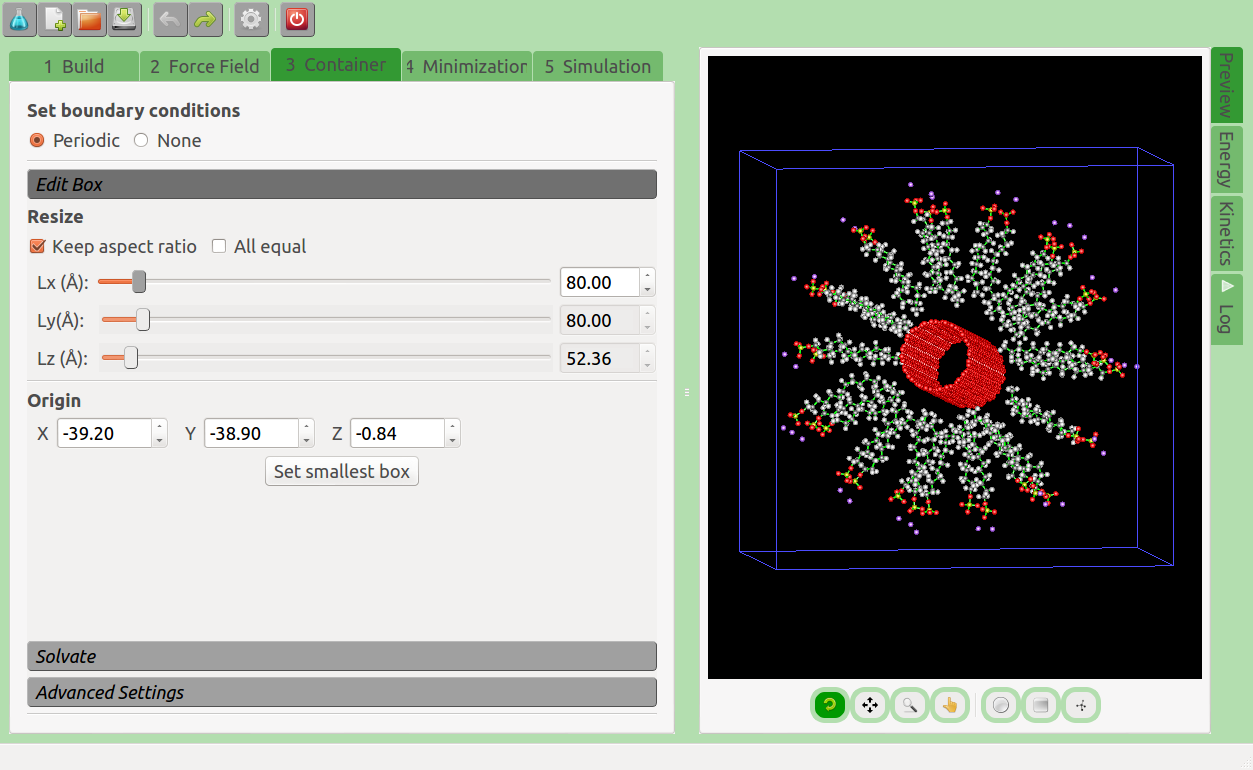
\includegraphics[scale=0.4]{setupTabA.png} \\
     (a)\\
  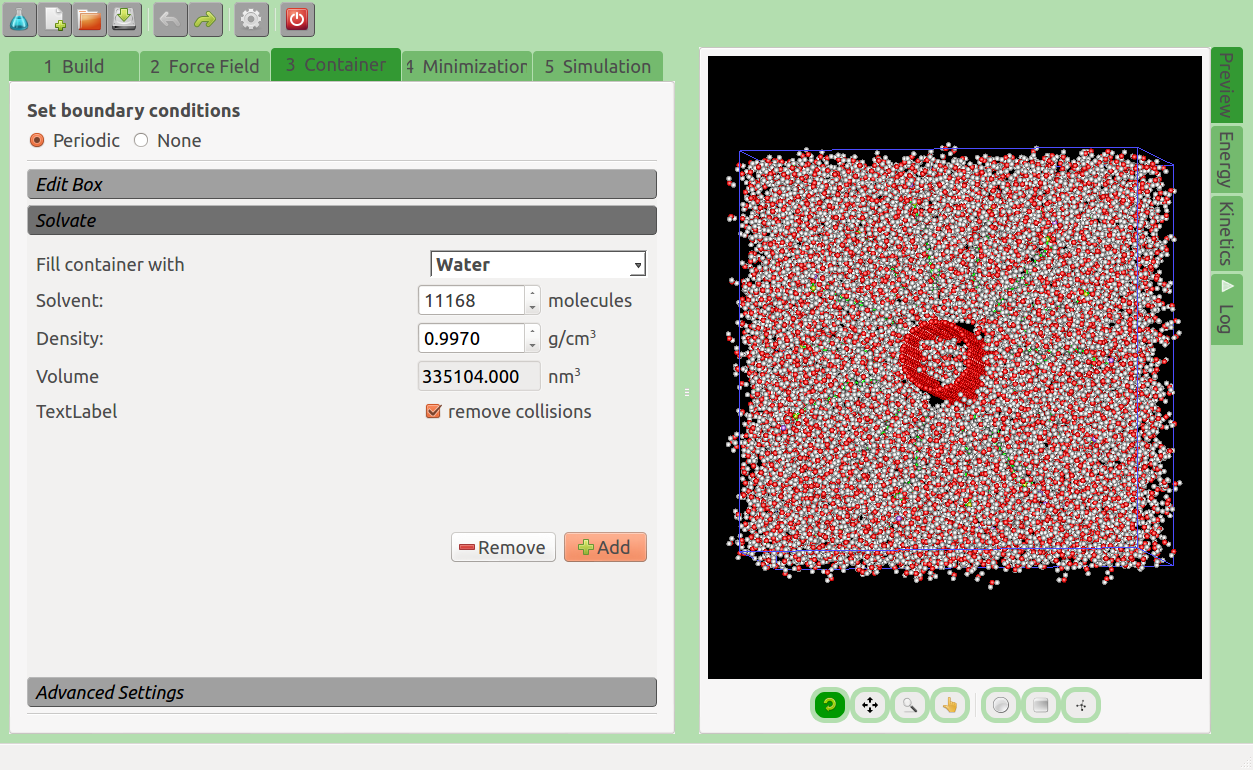
\includegraphics[scale=0.4]{setupTabB.png} \\
     (b) \\
  \end{tabular}
  \caption{The \textit{Container tab} with (a) a section for defining periodic boundary conditions and (b) a section for solvating the system.}

\end{center}
  \label{fig:setupTab}
\end{figure}

\subsection{Minimization tab.}  In Classical Molecular Dynamics the minimization step refers to finding a set of coordinates for the atoms in the system that represents a local potential energy minimum, usually by means of some kind of steepest descent method.  Minimizing the mixture makes more likely that the simulations may start and run without stability problems. 

Figure \ref{fig:minimizationTab} shows the minimization tab with the CNT-SDS mixture being minimized using NAMD.  Drop down menus containing different parameters that the CMD simulator required to control the minimization and simulation are presented.  Default values appear if the user has not set different ones.  The user can see how the molecular structures change while the minimization is running and monitor the progress of energy measurements with graphs which are updated while the minimization runs as well.  A linear fit is also drawn to suggest the tendency of the shown measurement to increase or decrease.  As a minimization progresses toward a potential energy minimum other energy measurements may increase.  Therefore the minimization should be performed until those measurements stabilize.  


\begin{figure}
\begin{center}
  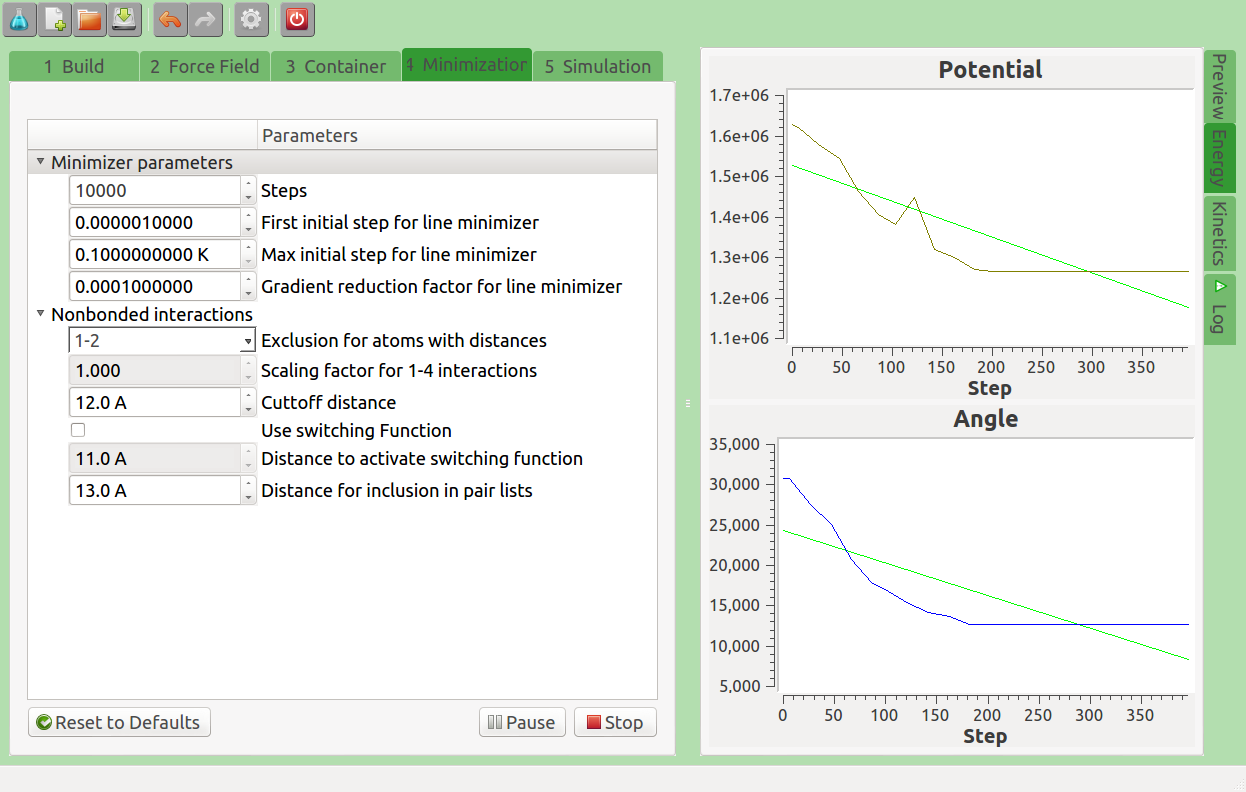
\includegraphics[scale=0.4]{minimizationTab.png} 
  \caption{The \textit{Minimization tab} showing the tendency of different energy measurements as the process progresses.}
  \label{fig:minimizationTab}

\end{center}\end{figure}



\subsection{Simulation tab.}  The molecular dynamics simulation is controlled from this tab.  A set of menus let the user define the parameters that control the simulation.  Consistency between parameters is enforced at the moment in which the user sets the values, before the simulation is submitted to the simulator.  For example, if the neighbor list radius is set smaller than the non-bonded cut-off radius, the user is informed immediately about the problem and an appropriate value is set.

Graphs with kinetics measurements (temperature, pressure, etc.) can be monitored as well during the simulation.  Clicking on a graph toggles the measure that is shown.  The information in these graphs is mostly used to determine when a simulation has stabilized.  But this mechanism also serves as an experimentation tool to determine appropriate values for some settings.  

For example, a rule of thumb used by MD scientists recommends setting the time step to ``\textit{approximately one-tenth the time of the shortest period of motion}"\cite{Leach1997} which should be reflected on the energy graphs.  
Figure  \ref{fig:simulationTab} shows two simulation tabs for an all atom model of chloroform and a model with no hydrogen \cite{Lukyanov2010}, respectively.
When small enough time step values are set oscillation patterns are clearly shown.  The smallest periods of motion for the models of 10 fs and 0.4 fs, respectively can be easily read from the graphs.  According to the rule of thomb mentioned above, this implies that with the second model the user can set a timestep value of one femto second, that is, 25 times higher with the no hydrogen model.


Figure \ref{fig:result} shows the CNT-SDS mixture being simulated in \textit{Wolffia}.  The usability features of the software allow the researcher to experiment with simulation settings in order to find the ones that better fit the characteristics of the mixture and produce stable simulations.  Once those settings 
are found and equilibration runs have been done using \textit{Wolffia}, all configuration packages can be packed in a zip file and transferred to a high performance server for a production run if needed.  
The final coordinates produced by those simulation runs may be imported into \textit{Wolffia} to update the information of the mixture.

\begin{figure}
\begin{center}
  \begin{tabular}{c}
  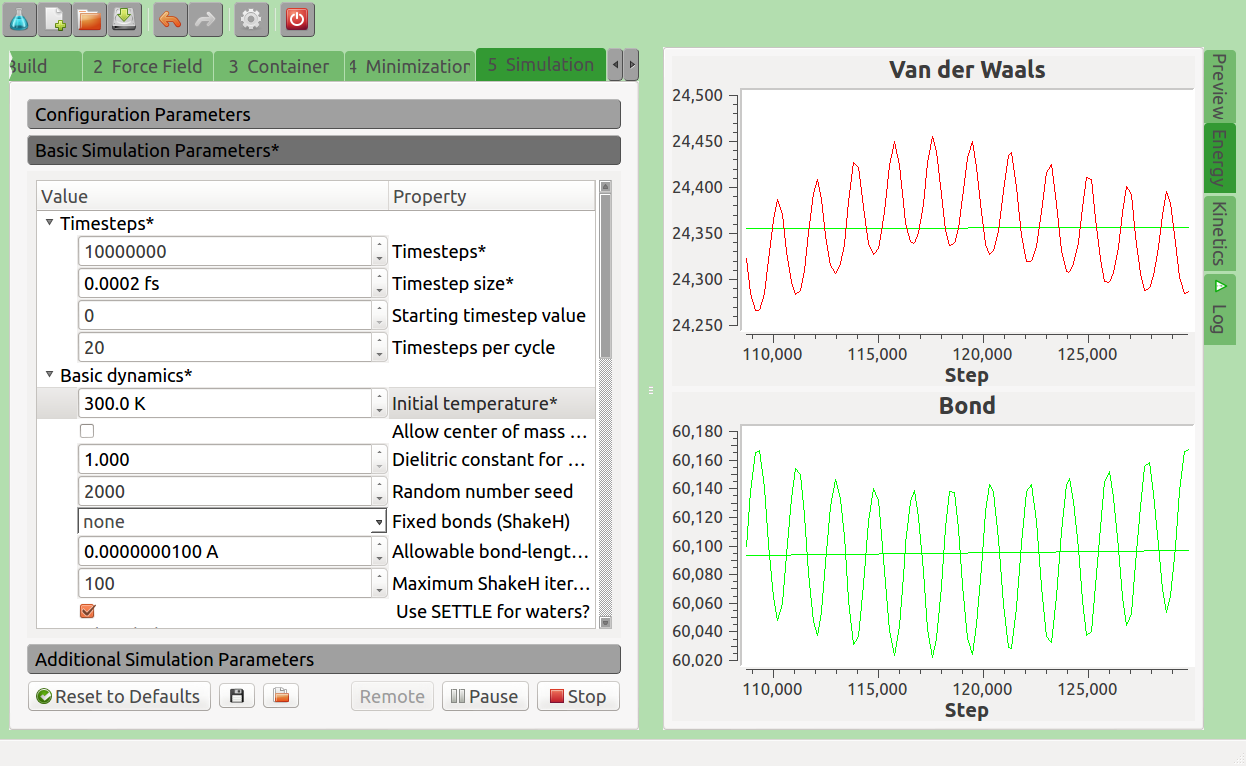
\includegraphics[scale=0.4]{simulationTabA.png} \\
  (a) \\
  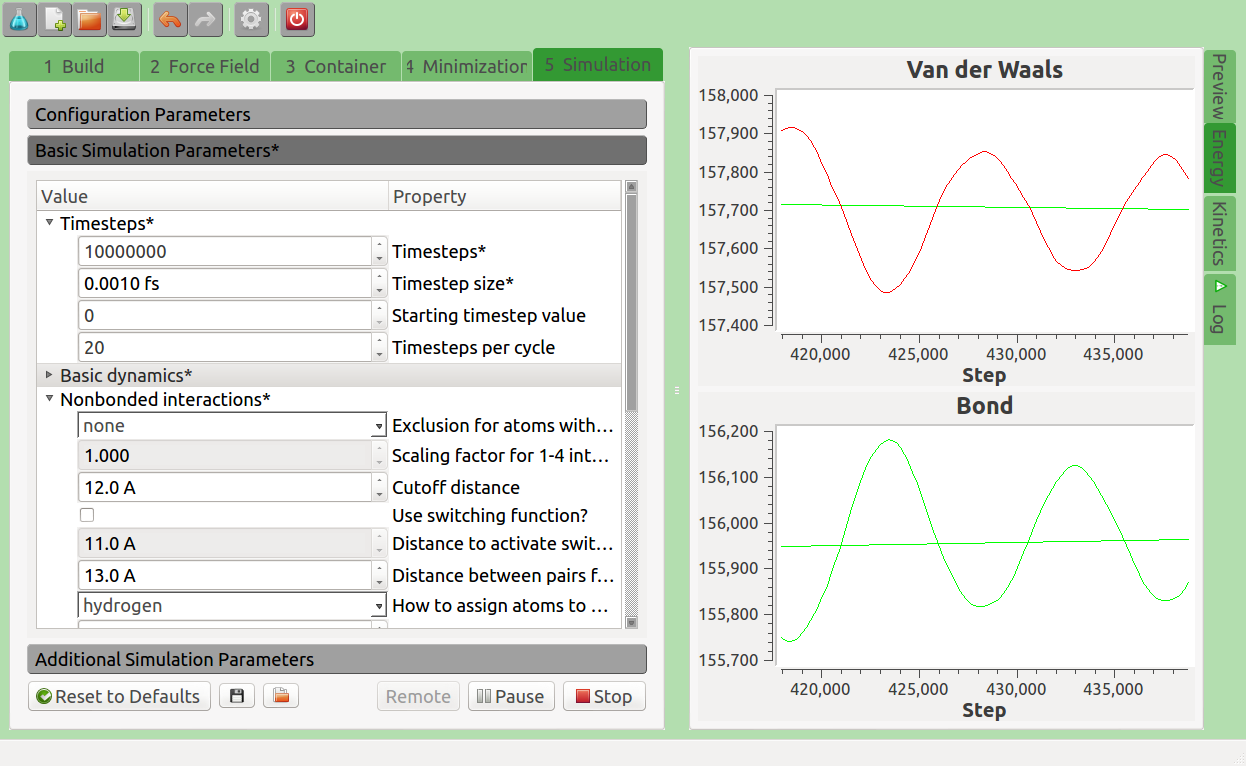
\includegraphics[scale=0.4]{simulationTabB.png} \\
  (b) \\
  \end{tabular}
  \caption{The \textit{Simulation tab} showing periodic variation of energy measurements of an all atom model of chloroform (left) and a model without hydrogen (right).}
  \label{fig:simulationTab}

\end{center}\end{figure}

\begin{figure}
\begin{center}
  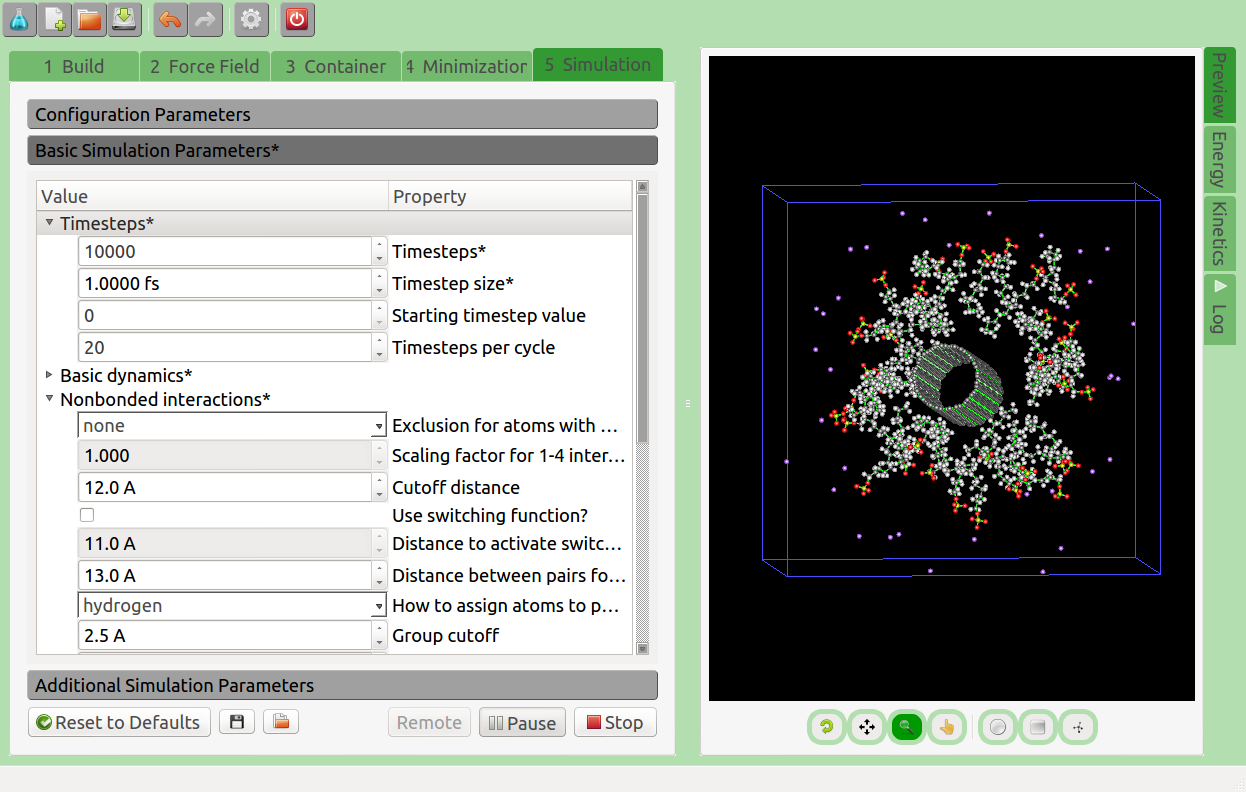
\includegraphics[scale=0.4]{result.png} 
  \caption{CNT-SDS mixture after a one nanosecond simulation (solvent hidden from view).}
  \label{fig:result}

\end{center}\end{figure}


\subsection{A test case}


Figure \ref{fig:testCase} illustrates the steps that a researcher may follow to simulate a single-strand DNA consisting of ten Cytosine bases (Poly-C). After a new empty mixture is created the \textit{Build tab} is presented to start the process (\ref{fig:testCase} (a)).  
The \textit{Graphene Editor} found in the \textit{Molecular Structure Catalog} is used to create a graphene sheet (\ref{fig:testCase} (b)).  A hole of about 30 {\AA} in diameter is made in the graphene using the \textit{hole tool} of the \textit{Molecule previewer} (\ref{fig:testCase} (c)).  
Then the Poly-Cyt Editor is used to create a 10-base molecule that is placed perpendicularly on top of the hole using the Properties Editor (\ref{fig:testCase} (d)). Sodium and Chlorine ions are added as well.
The force field parameter values can be inspected and customized using the Force Tab.  In this case, since only molecules from the Molecule catalog have been used, this step is skipped.

Periodic boundary conditions are set in the \textit{Container tab} (\ref{fig:testCase} (e)).  A box that fits the graphene sheet (plus the length of a carbon-carbon bond) is defined with a height that makes the interaction between the DNA strand and its copies in adjacent boxes negligible.  The \textit{solvate dialog} is used to fill the box with water (\ref{fig:testCase} (e)).

In order to equilibrate only the water, both the graphene sheet and the Poly-C are fixed in place by clicking on their corresponding \textit{pin widgets} in the build tab (\ref{fig:testCase} (f)).  Then a minimization is set and run in the \textit{Minimization tab} until the graphs of the energies flatten out (\ref{fig:testCase} (g)).  A 30k step simulation follows to finish the equilibration (\ref{fig:testCase} (h)).

Now the Poly-C molecule is set loose.  The menus in the \textit{Simulation tab} are used to set a 300K  initial temperature that is maintained using the Langevin temperature control.  An appropriate electric field perpendicular to the graphene sheet is set and particle mesh Ewald full electrostatics is selected.  A short simulation is performed to test the readiness of the system for a production CMD run.  The files necessary to run the simulation on a remote server are packed in a zip file in the \textit{Mixture Manager} dialog.  The files are transferred to the server and a 10ns simulated time production run is performed.  In our case an eight core system with four NVIDIA Tesla C2075 GPU processors running Ubuntu 12.04 64 bit server version OS and the multicore CUDA - capable NAMD version 2.9 taking 179 minutes to complete.  The coordinates of an intermediate step showing the strand passing through the nanopore were fed back into \textit{Wolffia} to update the system (\ref{fig:testCase} (i)).


\begin{figure}
\begin{center}
  \begin{tabular}{cc}
     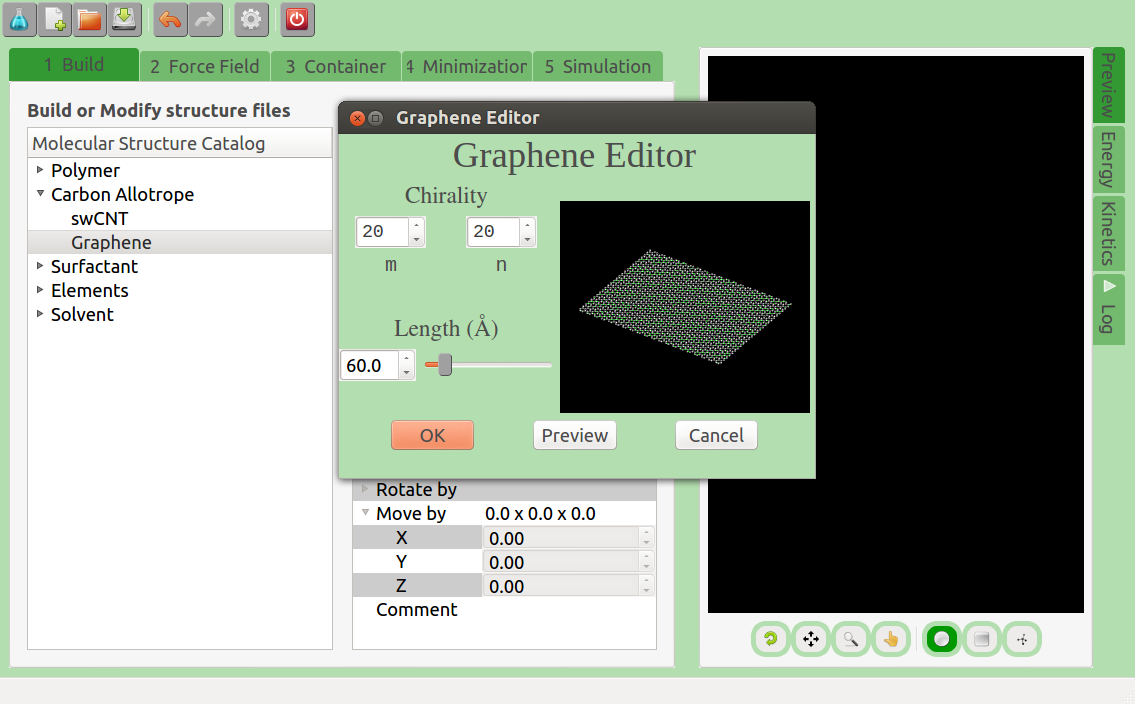
\includegraphics[scale=0.20]{01-Graphene.png} &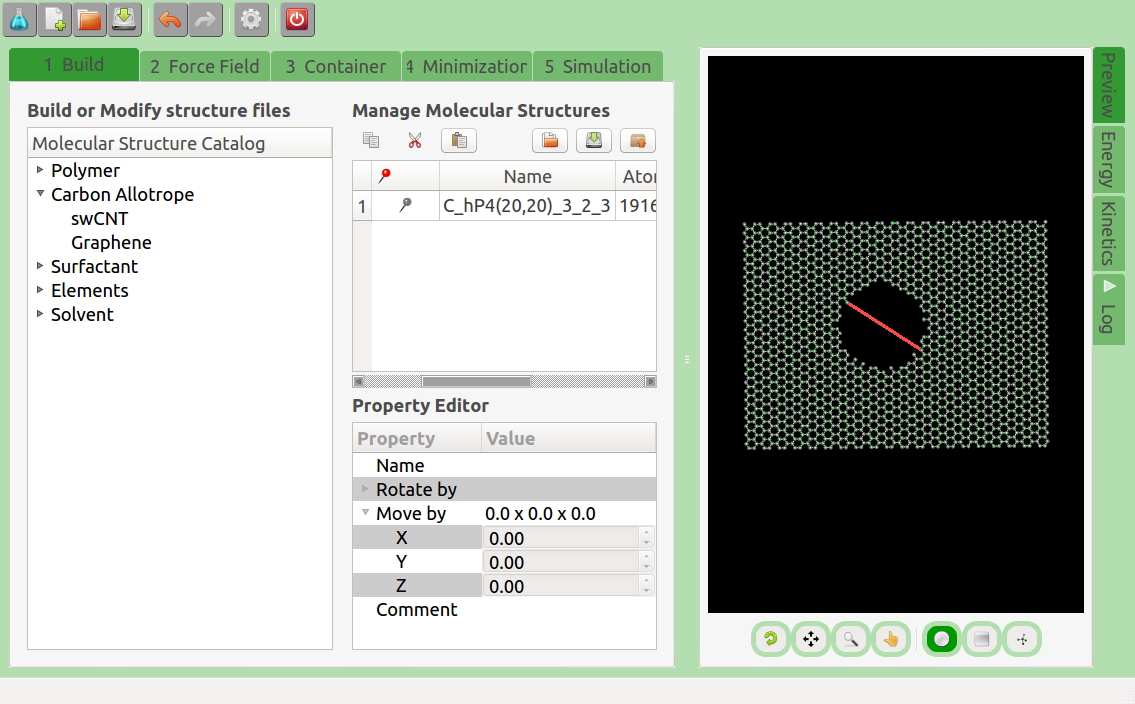
\includegraphics[scale=0.20]{02-Hole.png} \\
     (a) & (b)\\
      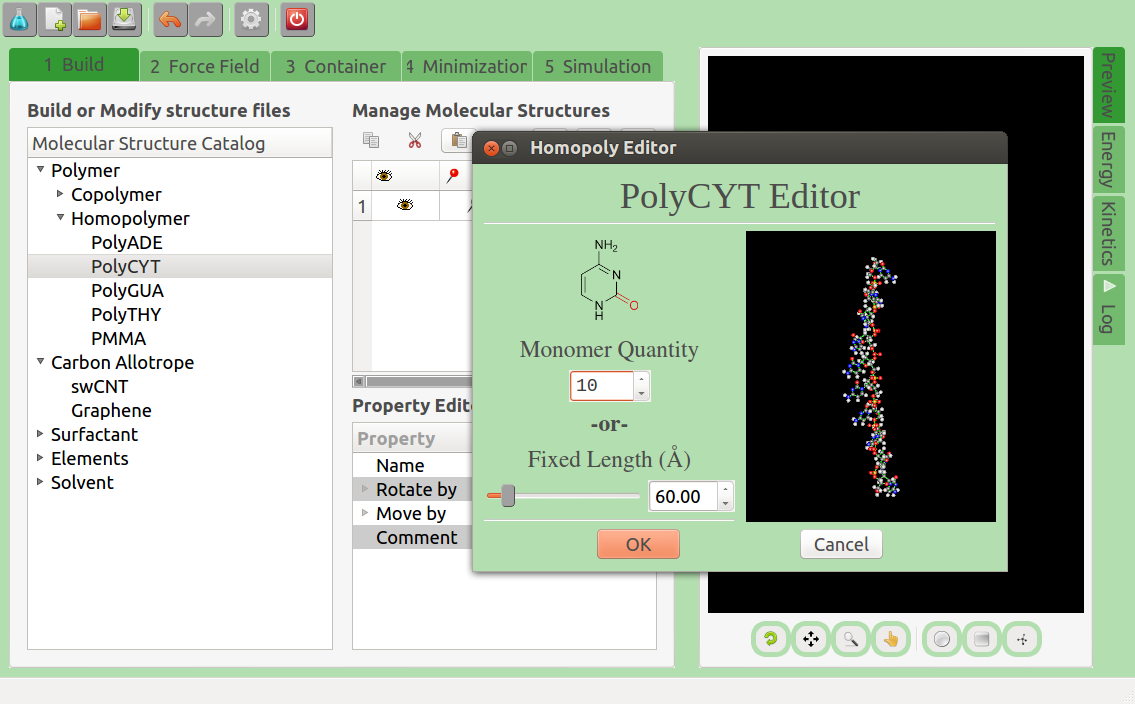
\includegraphics[scale=0.20]{03-PolyC.png} & 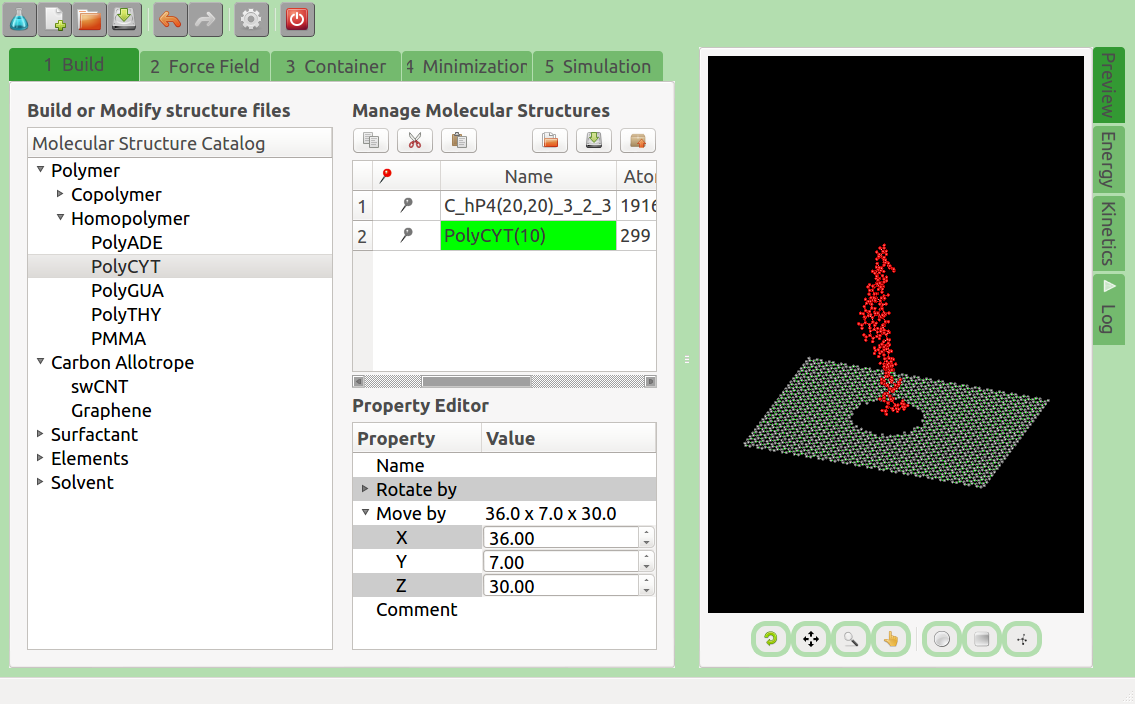
\includegraphics[scale=0.20]{04-Registering.png} \\
          (c)  & (d)   \\
       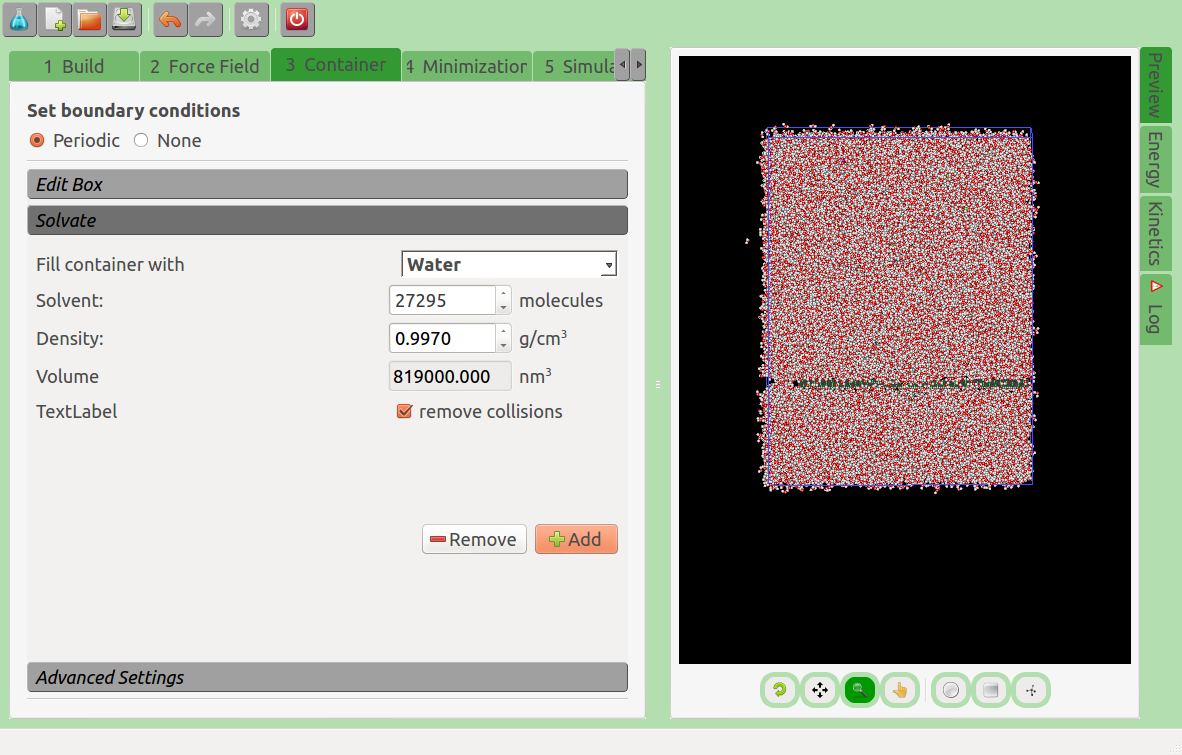
\includegraphics[scale=0.20]{05-Solvate.png} &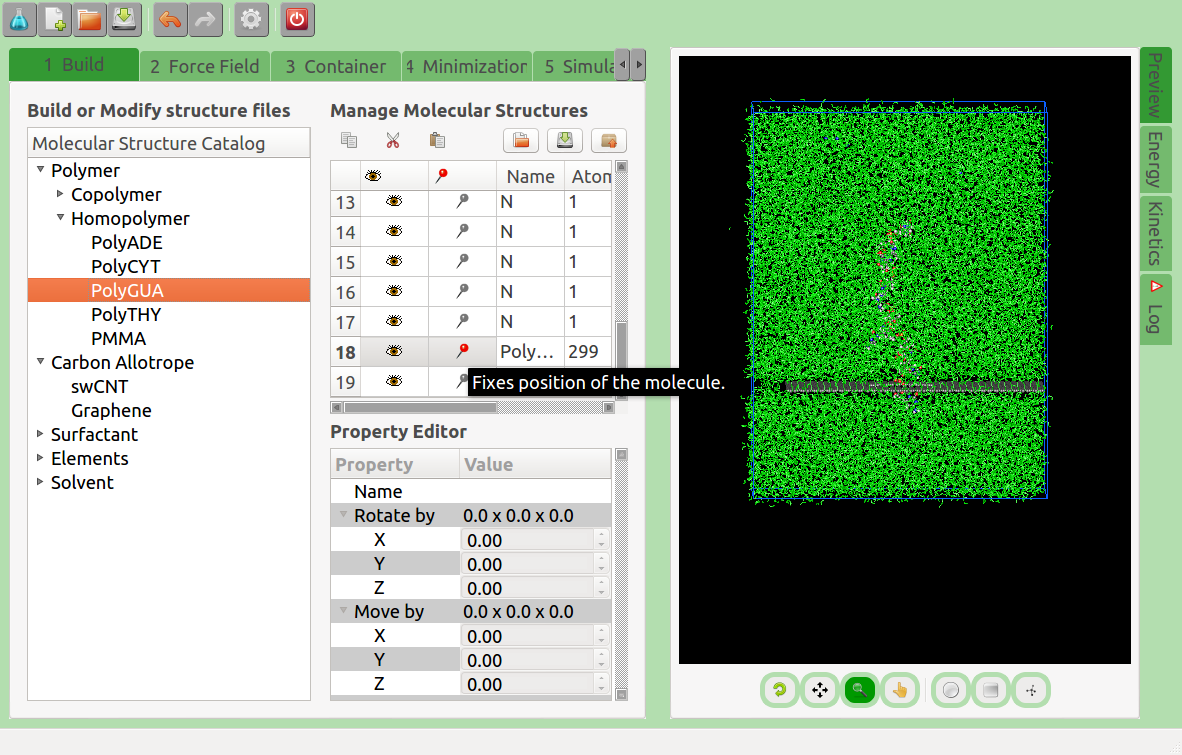
\includegraphics[scale=0.20]{06-Fixing.png}\\
     (e) & (f) \\
     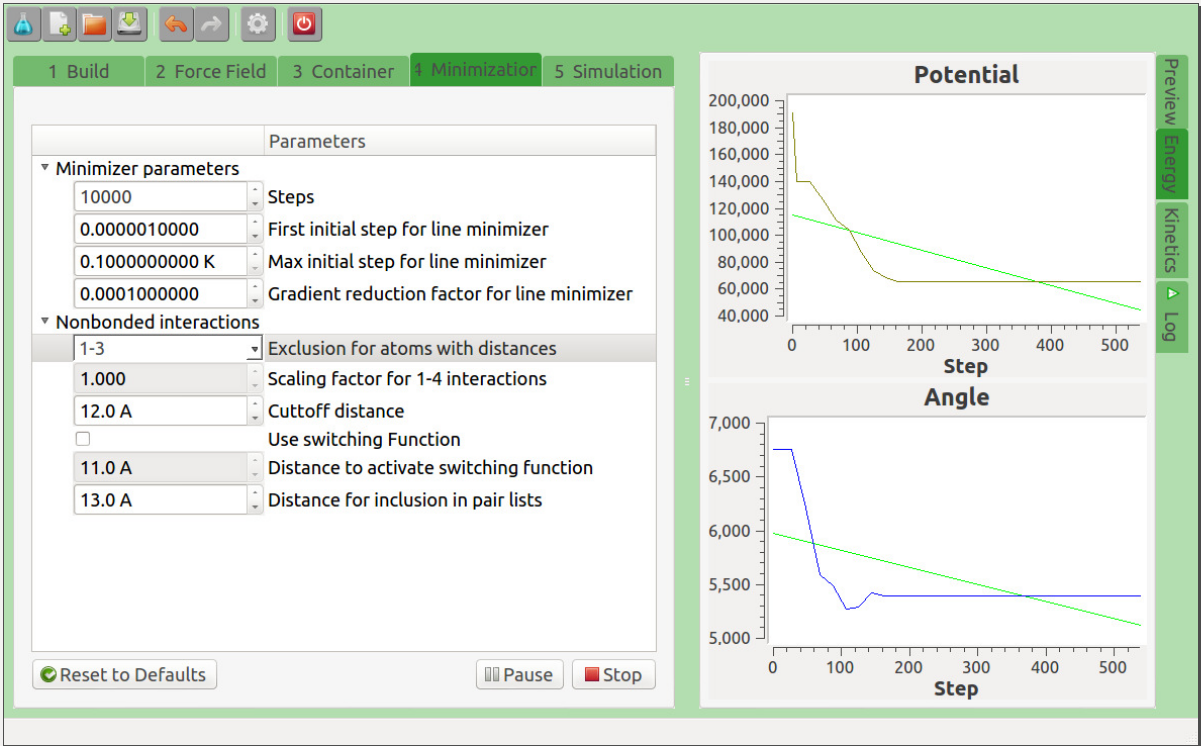
\includegraphics[scale=0.20]{07-Minimization.png} &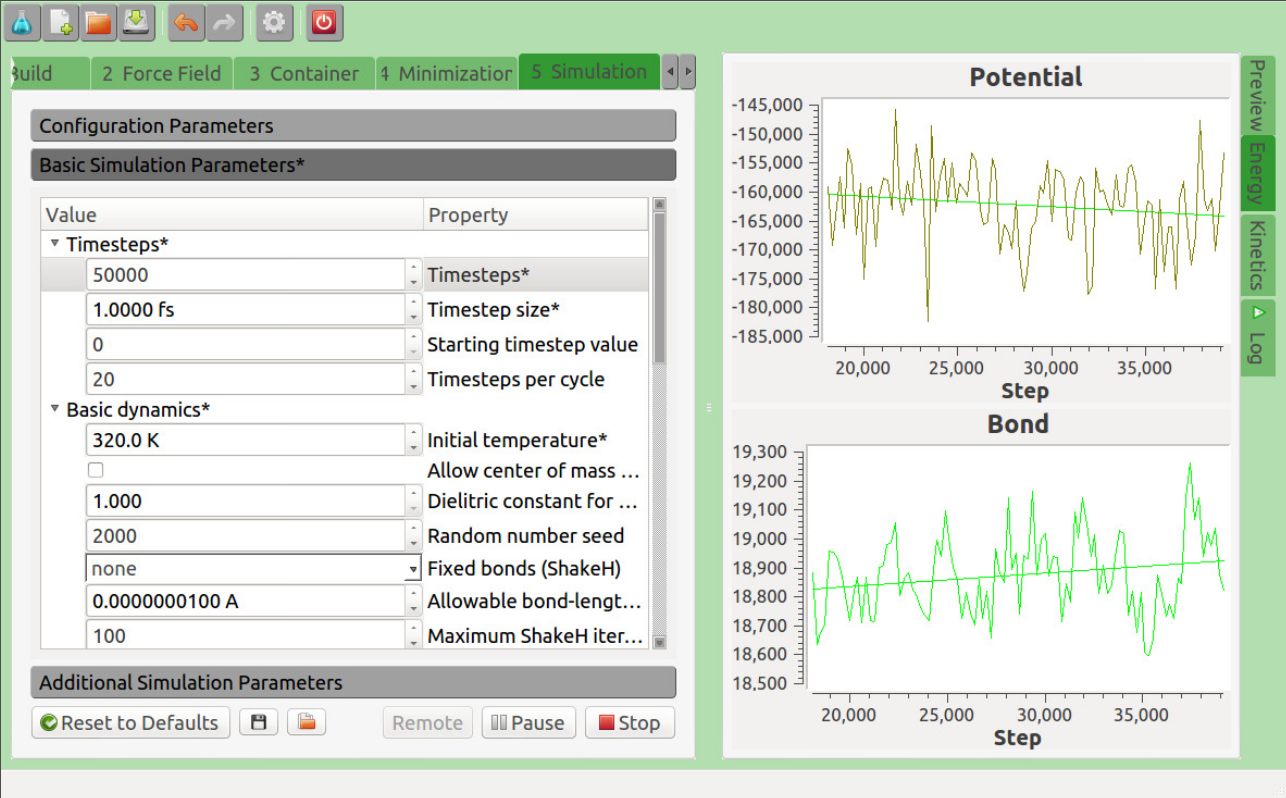
\includegraphics[scale=0.19]{08-Simulation.png} \\
     (g) & (h)\\
      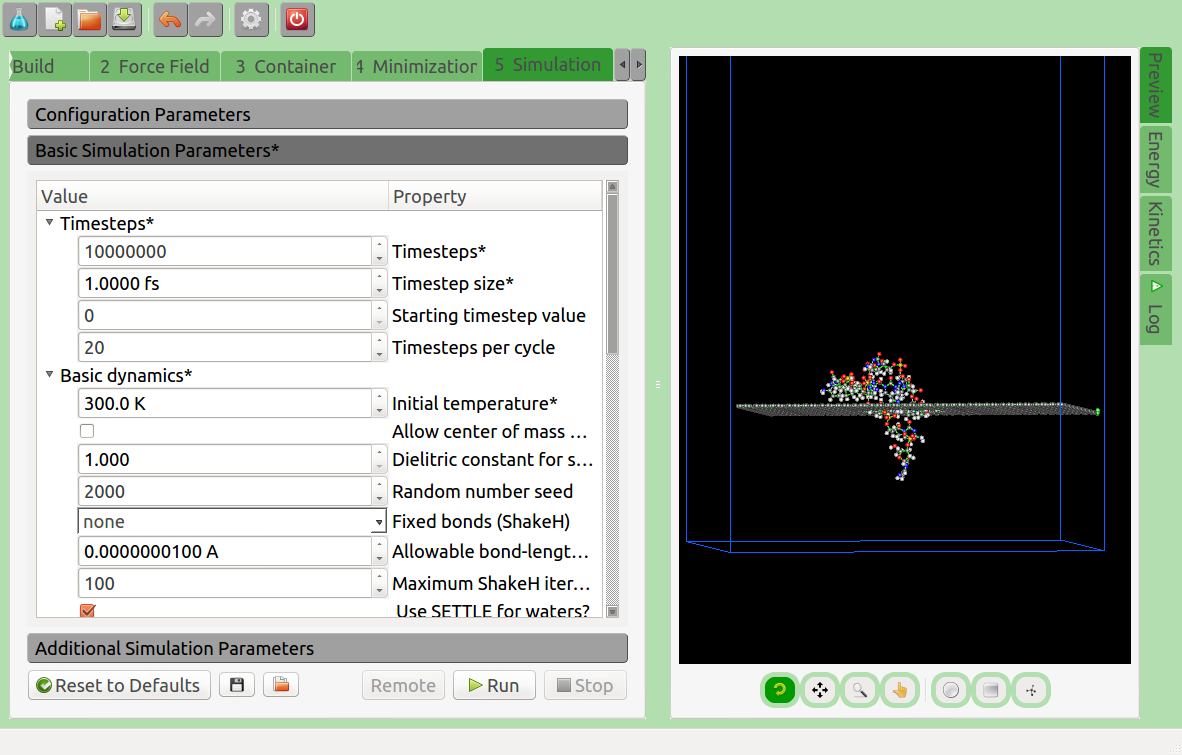
\includegraphics[scale=0.20]{09-Result.png}\\
      (i) \\
  \end{tabular}
  \caption{Setting-up and executing a molecular dynamics simulation using \textit{Wolffia}.}
  \label{fig:testCase}

\end{center}\end{figure}



\section{Implementation details.}  

\textit{Wolffia} has been written using the Python programming language.  Its graphical user interface was built using the PyQt\cite{PyQt}  Python bindings to the Qt GUI library.  The graphical representations of molecules are produced by the PyOpenGL\cite{PyOpenGL_openglpython}  interface to OpenGL.  This last aspect imposes some limitations on the size of the simulations that may be built in practice.  Because of that, \textit{Wolffia} provides a low resolution mode and an easy way to hide solvents, which most of the time account for most of the atoms in a mixture, to speed up drawings.  Also, since solvents are usually added last, this limitation should not be a problem to most users.  \textit{Wolffia} has been used successfully to build mixtures of more than 10k atoms (excluding solvents) and 100k atoms including solvents.

\textit{Wolffia} has been built on top of several open source libraries developed and maintained by active developing groups with recognized credentials on the applications being developed.
An object oriented library has been developed for the internal representation of molecules and mixtures on top of the \textit{NetworkX} software package for complex networks\cite{NetworkX} developed by Hagberg \textit{et.al.} at Los Alamos National Laboratory, USA.  Therefore, molecules and mixtures may be subject to analysis and experimentation using a large set of well tested graph theory methods provided by that package.  Coordinate files are managed by means of the Pybel wrapping of the OpenBabel cheminformatics toolkit\cite{Pybel}.

A description of the underlying software developed for this project, including the class hierarchies that describe how mixtures and molecules in the chemicalGraph module are derived from NetworkX classes and how basic \textit{Wolffia} widgets are derived from classes in the PyQt package can be found in a recent publication\cite{Wolffia01}.


\subsection{Installation requirements.}  \textit{Wolffia} was developed on the Ubuntu distribution of the LINUX operating system releases 11.04 through 12.10 (32 and 64 bits).  It has been been tested in the distributions of LINUX Debian 6.0, Mint 14 with KDE desktop environment,  and is expected to work on most Debian based LINUX distributions.  In those distributions the installation consists of executing two commands.  An rpm installation package is available an tested on Fedora 18.  There is also MS Windows version that has been tested on Windows XP and Windows 7.  The installation in these operating system requires the installation of Python and other Python packages.  Fortunately \textit{Python(x,y)} \cite{pythonxy} provides all of them in one package that is easy to install.  In all cases, NAMD has to be installed independently in order to run simulations.

Hardware requirements depend on the size of the systems to be built.  The test case shown in this paper was prepared using a laptop computer with an Intel I-7 Core processor and 4GB of RAM.






\section{Conclusion}

\textit{Wolffia} is the first open-source graphical user interface to a well established CMD simulator.  It provides support for the process of building a successful simulation.  Human Computer Interface principles served as a guide for its development and the implementation of them resulted in a user-friendly graphical user interface that helps the user in a easier and fastest way to assembly and monitor a CMD simulation.    Novice CMD simulators as well as experienced researchers may see the time required to set-up and run simulations significantly reduced.  As these types of computer simulations are being increasingly used in many fields of science, experimental groups may explore its applicability to their research by running their own small-scale simulations without getting involved in all the technical simulation details.

The use of open source libraries maintained by groups of researchers with recognized expertise in their subjects guarantees reliability and expandability.  It also provides a well developed and documented platform to programmers interested in further develop or customize the GUI.
The use of independent libraries has not implied difficult installation and update of the software.  On the contrary, installation and updates are easily performed in a couple of steps in Linux and Windows platforms.


%%%%%%%%%%%%%%%%%%%%%%%%%%%%%%%%%%%%%%%%%%%%%%%%%%%%%%%%%%%%%%%%%%%%%
%% The "Acknowledgement" section can be given in all manuscript
%% classes.  Rather than use \section, an appropriate macro is
%% provided that will always work.
%%%%%%%%%%%%%%%%%%%%%%%%%%%%%%%%%%%%%%%%%%%%%%%%%%%%%%%%%%%%%%%%%%%%%

\section{Acknowledgements}
This work has been supported by the \textit{National Science Foundation} under Grant NSF-DMR-0934195, \textit{PENN-UPRH Partnership for Research and Education in Materials} (PREM).

Wolffia has been developed by the \textit{Computational Science Group} of the Department of Mathematics, University of Puerto Rico at Humacao.  The following students are current participants in the project: Carlos Cort\'es, Melissa L\'opez  (currently a graduate student at the University of Puerto Rico, R\'{\i}o Piedras Campus), Frances Mart\'{\i}nez-Miranda, Radam\'es Vega Alfaro and Giovanni Casanova.
Student researchers testing simulations with Wolffia are   Wensy Cuadrado and Aixa de Jes\'us. 

The former student Mirgery Medina-Cuadrado (Curently at Universal Insurance Corp.) participated in its development and Rosely Qui\~nones tested force fields with the application.

Wolffia would not have been possible without the seminal work of the  former student researchers Myrna I. Merced-Serrano (currently at Southern Company), Axel Y. Rivera (currently a graduate student at the University of Utah), John E. Morales and Desiree Vel\'azquez.


%\end{acknowledgement}


%%%%%%%%%%%%%%%%%%%%%%%%%%%%%%%%%%%%%%%%%%%%%%%%%%%%%%%%%%%%%%%%%%%%%
%% The appropriate \bibliography command should be placed here.
%% Notice that the class file automatically sets \bibliographystyle
%% and also names the section correctly.
%%%%%%%%%%%%%%%%%%%%%%%%%%%%%%%%%%%%%%%%%%%%%%%%%%%%%%%%%%%%%%%%%%%%%

%\bibliographystyle{acm-sigchi}
%\bibliography{molecularDynamics}
\printbibliography

\end{document}